\SSbreak\\
\emph{Source: 2021 NICE Problem 10}\\
\emph{Proposer: \Pchan}\\ %\Pchan \Pbrain \Pss
\emph{Problem ID: 178}\\
\emph{Date: 2021-04-22}\\
\emph{Difficulty: Medium}\\
\SSbreak
 
\SSpsetQ{
    A circular sector of angle $\theta < 180^\circ$ is inscribed inside another sector of the same angle, shown below. If $\cos(\theta) = -\frac{m}{n}$, where $m, n$
    are relatively prime positive integers, find $100m + n$.

    \begin{center}
        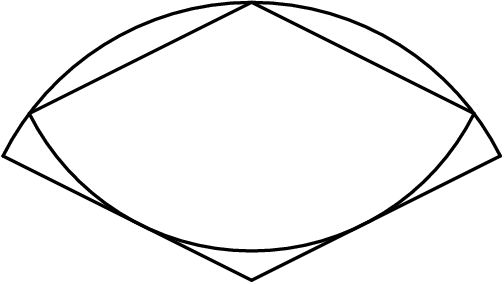
\includegraphics[scale=0.8]{Sections/Files/13-1-4.png}
    \end{center}
    %Put Problem Here
}\bigskip

\begin{solution}\hfil\medskip
	
    Let $r < R$ be the two radii of the sectors. Notice that the two red triangles shown below are both right triangles (one's a tangent, the other's the symmetry axis of an isosceles triangle)
    and one of their acute angles is $\frac{\theta}{2}$ in both triangles; since they share the same hypotenuse the two are congruent. Then by Pythagorean Theorem we have
    $$r^2 + \left(\dfrac{r}{2}\right)^2 = R^2 = \dfrac{5r^2}{4} \iff \dfrac{r}{R} = \dfrac{2}{\sqrt{5}} = \sin\left(\dfrac{\theta}{2}\right)$$
    so by double angle formula we have $$\cos(\theta) = 1 - 2 \sin^2\left(\dfrac{\theta}{2}\right) = -\dfrac{3}{5} \iff \boxed{305}.$$

    \begin{center}
        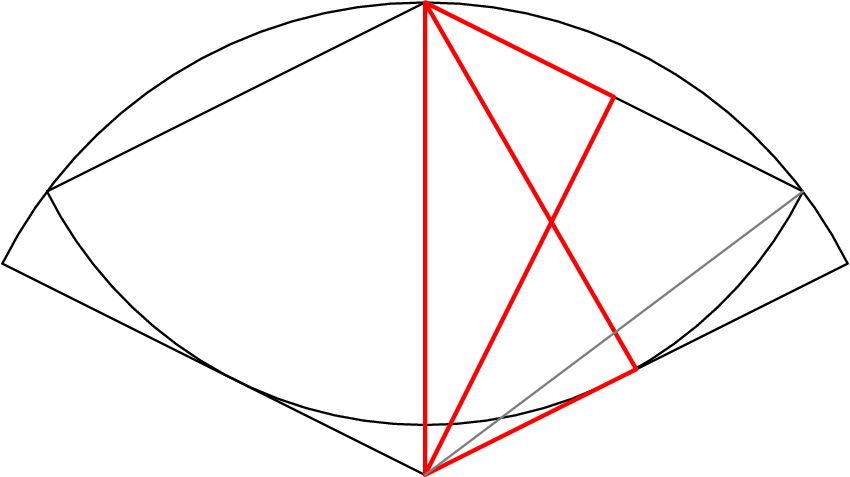
\includegraphics[scale=0.4]{Sections/Files/13-1-4S.png}
    \end{center}
    %Put sol here
\end{solution}\bigskip
